\documentclass[11pt]{article}
\usepackage[a4paper, margin=2cm]{geometry}
\usepackage[utf8]{inputenc}
\usepackage{babel}
\usepackage[spanish]{layout}
\usepackage[article]{ragged2e}
\usepackage{textcomp}
\usepackage{amsmath}
\usepackage{amssymb}
\usepackage{amsfonts}
\usepackage{proof}
\usepackage{enumerate}
\usepackage{graphicx}
\usepackage{multirow}
\usepackage{caption}
\usepackage{subcaption}

\setlength{\parindent}{0pt}

\title{
    Entrega 9 \\
    \large Sistemas Operativos II}
\author{Mellino, Natalia \and Farizano, Juan Ignacio}

\date{}

\begin{document}
\maketitle

\noindent\rule{\textwidth}{1pt}

\section*{Ejercicio 1}

\begin{figure}[h!]
  \begin{center}
    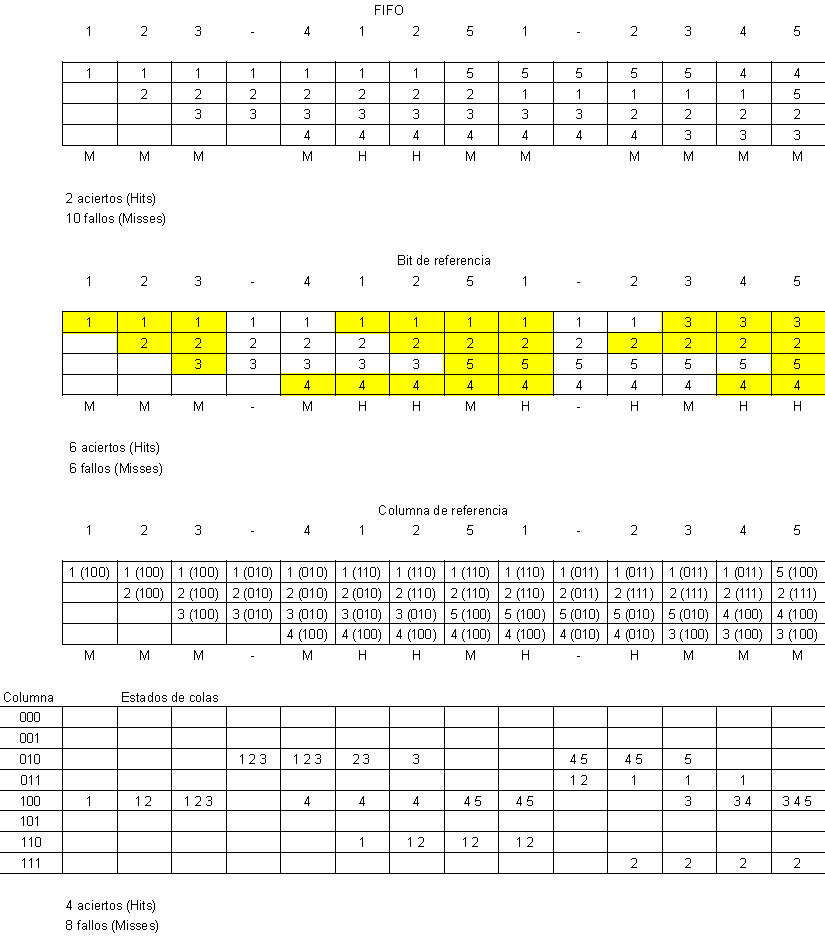
\includegraphics[width=0.99\linewidth]{Paginación.pdf}
  \end{center}
\end{figure}

\section*{Ejercicio 2}

Por lo general esta tarea es realizada por el hardware. Suponemos que específicamente
la MMU cuando se solicita una lectura o escritura de memoria.

\section*{Ejercicio 3}

Esta decisión se debe a un mecanismo que se emplea para hacer que el sistema busque
siempre tener espacio disponible en memoria en vez de esperar a que surja la necesidad
de reemplazar un marco marcado como escrito, resultando en una mayor latencia. Entonces, 
para hacer esto el sistema operativo busca las páginas sucias más proclives a ser 
llevadas a disco (siempre que sea posible) y va actualizando la imagen en disco,
borrando el bit de escritura.

\section*{Ejercicio 4}

\begin{itemize}
\item No es posible. Al no haber ningún mecanismo de memoria compartida, no existe
la posiblidad de que dos o más procesos carguen la misma página en memoria, 
porque no la están compartiendo en un principio. Y no es posible que un solo
proceso cargue dos veces la misma página de la swap, ya que va a estar bloqueado
esperando que la página se cargue a memoria.

\item Si, es posible. Como es el sistema el que decide enviar una página a swap, un proceso
puede intentar utilizar esta página antes de que se efectivice la escritura (realizada
por el sistema) ocasionando que se traiga del disco una versión anterior de la página.
\end{itemize}

\section*{Ejercicio 5}

\begin{itemize}
  \item A diferencia de paginación, rastrear la memoria libre/usada resulta más sencillo.
  \item Es posible ceder grandes bloques de memoria contiguos para los procesos que
        lo necesiten, como por ejemplo los controladores de DMA.
  \item No se produce fragmentación externa ya que los bloques liberados tienen la 
  posibilidad de fundirse.
  \item Poco desperdicio de memoria (a lo sumo la mitad de un bloque, ya que si 
  fuera más pequeño, se pediría un bloque más pequeño).
  \item El Slab Allocator contribuye a reducir la fragmentación interna ya que este actúa
  cuando hay pedidos de memoria demasiado pequeños (menor a una página).
\end{itemize}

\end{document}